%\vspace{-0.1in}
\section{\sysname{} for Clos Topology}
\label{sec:specific}

\begin{figure}[t]
		\centering
		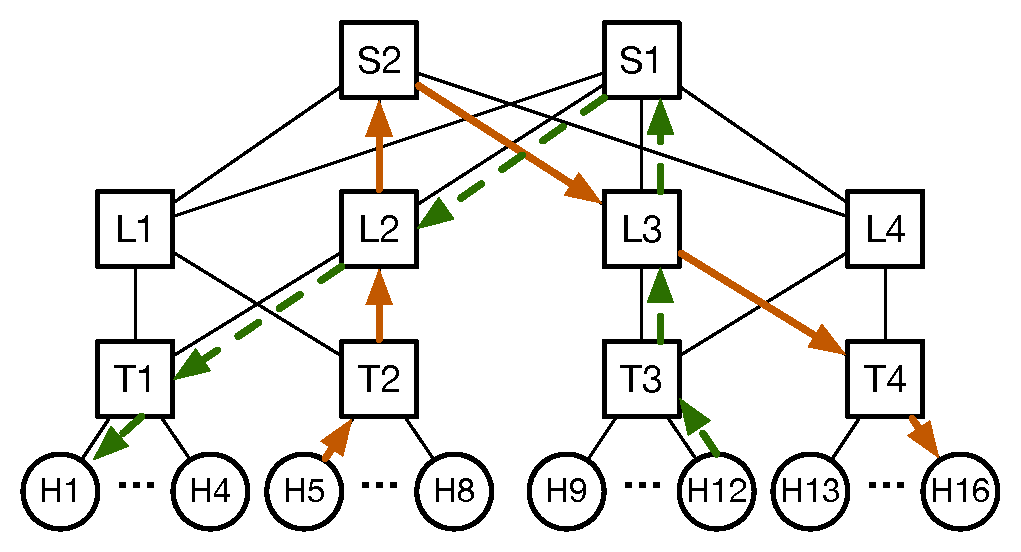
\includegraphics[width=0.3\textwidth] {figs/updown_paths}
		\caption{Clos topology with two flows following up-down .}
		\label{fig:basic_clos}
\end{figure}

While \sysname{} works for any topology, we first describe the core ideas using
the popular Clos network topology.

\subsection {Definitions}

\para{Expected Lossless Paths (ELP):} This is a set of paths that the network
operator requires to be lossless. For example, in a Clos network, the operator
may want that all up-down paths or all shortest paths to be lossless.  Any route
can be included in ELP, as long as it does not have a loop.

\para{Lossless class:} A lossless class is a service that the network provides for
applications. The network guarantees that packets in a lossless class will not
be dropped due to buffer overflow as long as they traverse paths in ELP.

\para{Tag:} Tag is a small integer assigned / associated with a packet. The tag
is embedded in a packet. A packet belonging to one lossless class may change its
tag value, which means that a lossless class may have multiple tag values.

\para{Switch model:} For ease of discussion, we use a simplified
switch model in this section.  A switch has multiple ports. Each port has up to 7
lossless queues associated with it, and one lossy queue\footnote{All queues
share a single packet buffer.}. The queue number corresponds to the PFC priority.
Switch classifies arriving packets into queues based on {\em tags}.  Typically,
each tag maps to a single priority value. If a tag does not match any priority
value, the packet is added to a lossy queue. Before forwarding a packet, the
switch can rewrite the tag according to user-specified rules.

We now describe the core idea behind \sysname{}.

\subsection{Tagging on bounce}
\label{subsec:tag}

Consider Figure~\ref{fig:basic_clos}. Lets assume that the operator defines ELP
simply - just shortest up-down paths as they exist in this network.  Both the
green and blue flows follow such paths and there is no deadlock.

Now, let's assume that as shown in Figure~\ref{fig:clos_1_bounce}, two links
fail, which forces both flows to travel on paths that are not in the ELP. We
call these paths 1-bounce paths, as the path violates the up-down rule once
($L2$ to $S1$ for green flow, $L3$ to $S2$ for blue flow). As shown, this can
lead to CBD, and hence may cause deadlock.

One way to avoid such CBD is to put any packets that have deviated from the ELP
 in a lossy queue.  Being assigned to lossy queue means that such packets
will not trigger PFC. Since the paths in ELP are shortest up-down paths they are
deadlock free, and the bounced packets won't trigger PFC, the network will stay
deadlock free even if packets bounce.

We stress that being assigned to lossy queue does not mean that the packets are
immediately (or ever) dropped -- they are dropped {\em only if} they arrive at a
queue that is full. The only thing we need is that these packets do not trigger
PFC.

Thus, if each switch can detect that an arriving packet has traveled (sometime
in past) on a non-ELP, it can put the packet in lossy queue, and there will be
no deadlock.

How can a switch determine whether the packet has bounced, using just local
information, in presence of dynamic routing?

Consider the green flow in Figure~\ref{fig:clos_1_bounce}.  We want switch $S1$,
the first switch after bounce, to detect the bounce and put the packet in a
lossy queue.

One way for $S1$ (and any other switch afterwards) to recognize a bounced packet
is by TTL. Since the ELP consists of shortest paths, a bounced packet will have
``lower than expected'' TTL. However, TTL values are set by end
hosts\footnote{TTL has other issues as well, see \S\ref{subsec:caveats}}, so a
more controllable way is for the switch $L2$ to provide this information via a
special tag (e.g. DSCP value) in the packet. Note that for any ELP path, $L2$
would have never forward any packet that arrived from $S2$ to $S1$. So, if $L2$
``tags'' packets that have arrived from $S2$ that it is forwarding to $S1$, then
$S1$, {\em and all other switches along the path after $S1$} know that the
packet has travelled on a non-ELP path.

Note that $L2$ needs only local information to do the tagging. We can initially
assign a $NoBounce$ tag to every packet. $L2$ then simply needs to check ingress
and egress port for each packet: it changes the tag from $NoBounce$ to $Bounced$
if a packet arriving from ingress port connected to $S2$ exits on egress port
connected to $S1$.  It is easy to see that these rules can be pre-computed since
we know the topology, and the set of  that we want to be ``lossless''.

This, in essence, is the core idea behind \sysname{} -- given a topology and ELP
we can create a system of tags and {\em static} rules that manipulate these tags
to ensure that there will not be CBD, even when the underlying routing system
 packets on paths that are not in the ELP.

Of course, this basic idea is not enough. First of all, packets may bounce not
just from the Leaf layer, but at any layer. Second, recall from
\S\ref{sec:reroute} that ``bounces'' are a fact of life in data center networks.
The operator may not want to put packets that have suffered just a single bounce
into a lossy queue -- we may want to wait until the packet has bounced more than
once before assigning it to a lossless queue. This means that ELP will consists
of more than shortest up-down paths, and the paths in ELP may be prone to CBD!
Third, we must ensure that we
don't end up using more lossless queues than the switch can support. To this
end, we show how to combine tags.

\begin{figure}[t]
	\centering
	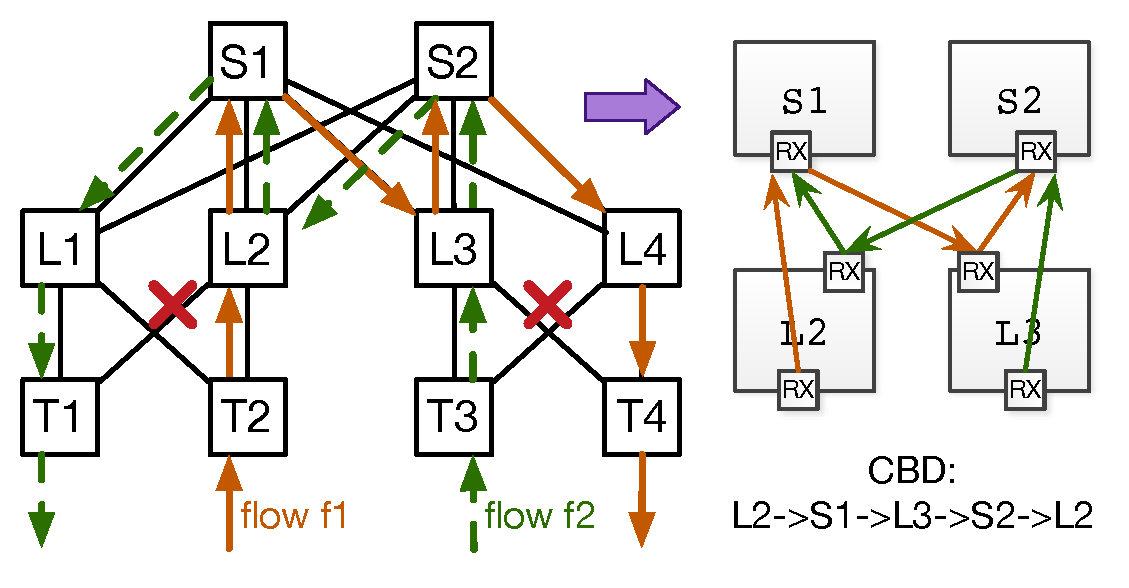
\includegraphics[width=0.5\textwidth] {figs/cbd_a}
	\caption{1-bounce path creates CBD.}
	\label{fig:clos_1_bounce}
\end{figure}

\subsection{Reducing the number of lossless queues}
\label{subsec:combine}

Consider again the network Figure~\ref{fig:basic_clos}.  Let's say the operator
wants to make sure that in face of link failures, packets are not immediately
put into a lossy queue. The operator is willing to tolerate up to $k$ bounces.
So, the ELP consists of all shortest paths, and all paths with up to $k$ bounces.
Do we need to assign a distinct tag and a corresponding priority queue for each
bouncing point?

To answer this question, we leverage our knowledge of Clos topology.  Consider a
packet that bounces twice. The path between the first bounce and the second
bounce is a normal up-down path. Therefore, these path segments do not have CBD
even if we combine them into a single priority queue. We can use a single tag to
represent these segments altogether, and map the tag to a globally unique
priority queue.

This completes the design of \sysname{} for Clos topology. Packets start with
tag of 1. We configure all ToR and Leaf switches such that every time they see
a packet coming down and then going up (therefore, bouncing) for any reasons,
they increase the tag by one. Spine switches do not need to change tags since 
packets never go up there.

All switches put packets with tag $i$ to $i^{th}$ lossless queues. Since ELP
includes paths with up to $k$ bounces, the switches need to have $k+1$ lossless
queues. If a packet bounces more than $k$ times (e.g. due to numerous link
failures, or loop), it will carry a tag larger than $k+1$. All switches will put
such packets into a lossy queue.  Pseudocode of the algorithm, using notation
developed in \S\ref{sec:generic}, is shown in Appendix~\ref{sec:clos_optimal}.

Figure~\ref{fig:clos_tagger} illustrates the tagging algorithm in action, for
ELP consisting of all shortest up-down paths, plus all 1-bounce paths.
Packets, when traveling on path segments before bounce carry a tag value of 1,
and the tag is set to 2 after the bounce. This ensures that the packets are
queued in separate lossless queues, and thus there is no CBD. In other words, we
show a system for $k=2$. The lossy queue for packets that bounce more than once
is omitted for clarity. The corresponding tag rewriting rules at  $T2, L2 and
S2$ are shown in Table~\ref{tab:clos_tag_rules}.  Rules for other switches are
similar. Note that only $L2$ is doing any ``rewriting''.
\S\ref{sec:implementation} we will show how to implement these rules compactly
using TCAM match-action tables.

This design satisfies all three challenges described in \S\ref{sec:challenges}.
We do not change the routing protocol. We work with existing hardware. We deal
with dynamic changes to , and we do not exceed the number of available
lossless queues.

\begin{figure}[t]
	\centering
	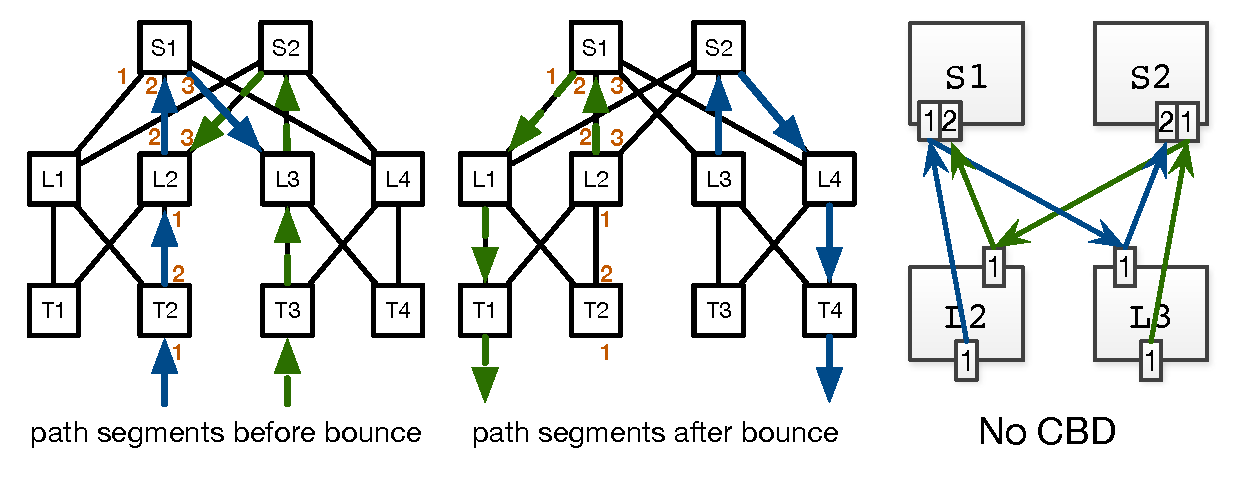
\includegraphics[width=0.5\textwidth] {figs/cbd_b}
	\caption{Illustration of \sysname{} for ELP of all shortest up-down paths,
		and all 1-bounce paths. For clarity, only lossless queues are shown.}
	\label{fig:clos_tagger}
\end{figure}

\begin{table}[t]
		\centering
		\footnotesize
		\begin{tabular}{l}
		\begin{tabular}{|r|r|r|r|}
			\hline
			Tag&  Ingress& Egress & Newtag \\
			\hline
			\hline
			1 & 1 & 2 & 1 \\
			\hline
			\multicolumn{4}{c}{(a) At switch T2} \\
		\end{tabular}
		\\
		\begin{tabular}{|r|r|r|r|}
			\hline
			Tag&  Ingress& Egress & Newtag \\
			\hline
			\hline
			1 & 1 & 2 & 1 \\
			\hline
			1 & 3 & 2 & \textcolor{red}{2} \\
			\hline
			\multicolumn{4}{c}{(b) At switch L2} \\
		\end{tabular}
		\\
		
		\begin{tabular}{|r|r|r|r|}
			\hline
			Tag&  Ingress& Egress & Newtag \\
			\hline
			\hline
			1 & 2 & 3 & 1 \\
				\hline
			\textcolor{red}{2} & 2 & 1 & \textcolor{red}{2} \\
			\hline
			\multicolumn{4}{c}{(c) At switch S1} \\
		\end{tabular}
		
	\end{tabular}
		\caption{Tag rewriting rules for $T2$, $L2$ and $S1$ for Figure~\ref{fig:clos_tagger} to support
		ELP of all shortest up-down paths, and all 1-bounce paths. Rules on other
		switches are symmetric.}
		\label{tab:clos_tag_rules}
		\vspace{-1em}
\end{table}

\subsection {Deadlock freedom and optimality}
\label{subsec:specific_deadlock_free}

We now provide brief proof sketches to prove that the above algorithm is
deadlock free, and optimal in terms of number of lossless priorities used.

%% \begin{figure}[t]
%% 	%\vspace{-0.1in}
%% 	\centering
%% 	
%% 	\subfloat[short for lof][CBD across subspaces.] {
%% 		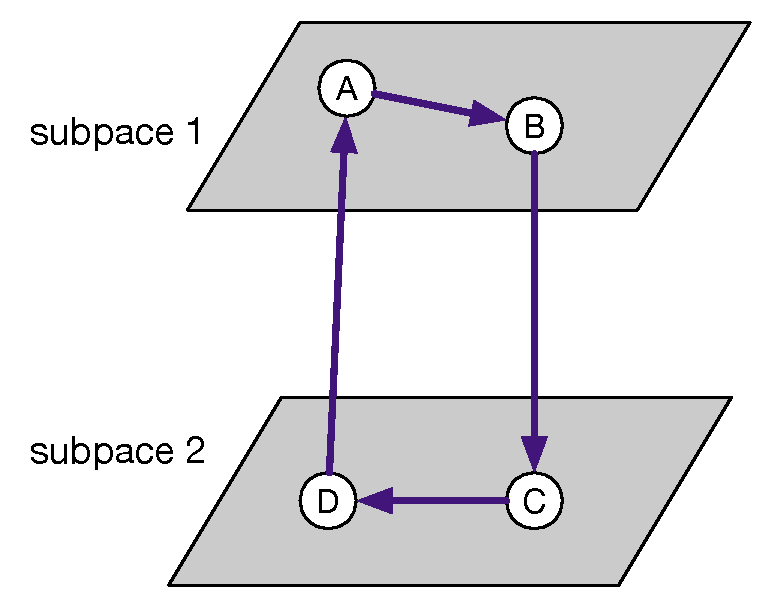
\includegraphics[width=0.26\textwidth] {figs/subspace_a}
%% 	}
%% 	\subfloat[short for lof][DAG across subspaces.]{
%% 		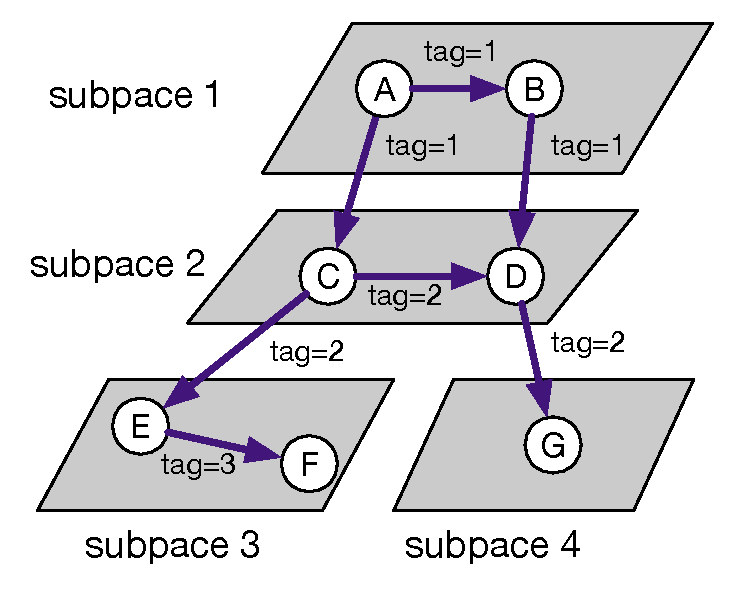
\includegraphics[width=0.24\textwidth] {figs/subspace_b}
%% 	}
%% 	
%% 	\caption{DAG across subspaces ensure deadlock-free priority transition.}\label{fig:subspace}
%% \end{figure}

\para{\sysname{} is deadlock-free for Clos networks:} \sysname{} has two
important properties. First, for any given tag and its corresponding priority
queue, there is no CBD because each tag only has a set of ``up-down'' routing
paths.  Second, every time the tag changes, it changes monotonically. This means
that the packet is going unidirectionally in a DAG of priority queues. This is
important because otherwise CBD may still happen across different priorities.
We conclude that no CBD can form either within a tag or across different tags.
The network is deadlock-free since CBD is a necessary condition for deadlock.  A
formal proof, which applies to any topology, is given in \S\ref{sec:generic}.
%(Figure~\ref{fig:subspace}). 

\para{\sysname{} is optimal in terms of lossless priorities used:} We show that
to make all $k$ bounces paths lossless and deadlock-free, at least $k+1$
lossless priorities are required. We use contradiction.  Assume there exists a
system with only $k$ lossless priorities. Consider a flow that loops between
$T1$ and $L1$ for $k+1$ times, which means it bounces $k$ times at $T1$. With
Pigeonhole principle, we know that at least two times during the looping, the
packet must have the same lossless priority. This is sufficient to cause
a deadlock~\cite{hu2016deadlocks}. Contradiction.

\subsection {Summary}

We showed that given a Clos topology and a set of  (up-down, plus up to $k$
``bounces'') that should be lossless, we can generate a system of tags and
associated rules that ensure that packets are correctly classified into $k$
lossless queues plus one lossy queue to ensure that there is no deadlock.   This system can be
implemented with existing hardware, without requiring any changes to the routing
protocol. We also showed that this system is optimal, in the sense that we
cannot prevent deadlock with fewer lossless queues.

Much of the discussion in this section used the specific properties of Clos
networks, and the specific ELP set. We now show how to generalize \sysname{} for
any topology and any ELP set.
